
\subsubsection{Soft-NMS}
NMS算法的大致过程可以看原文这段话:

First, it sorts all detection boxes on the basis of their scores. The detection box M with the maximum score is selected and all other detection boxes with a significant overlap (using a pre-defined threshold) with M are suppressed. This process is recursively applied on the remaining boxes.

那么传统的NMS算法存在什么问题呢?可以看Figure1。在Fiugre1中,检测算法本来应该输出两个框,但是传统的NMS算法可能会把score较低的绿框过滤掉(如果绿框和红框的IOU大于设定的阈值就会被过滤掉),导致只检测出一个object(一个马),显然这样object的recall就比较低了。 
可以看出NMS算法是略显粗暴(hard),因为NMS直接将和得分最大的box的IOU大于某个阈值的box的得分置零,那么有没有soft一点的方法呢?这就是本文提出Soft NMS。那么Soft-NMS算法到底是什么样呢?简单讲就是:

An algorithm which decays the detection scores of all other objects as a continuous function of their overlap with M.

换句话说就是用稍低一点的分数来代替原有的分数,而不是直接置零。另外由于Soft NMS可以很方便地引入到object detection算法中,不需要重新训练原有的模型,因此这是该算法的一大优点。

\begin{uscfigure}
	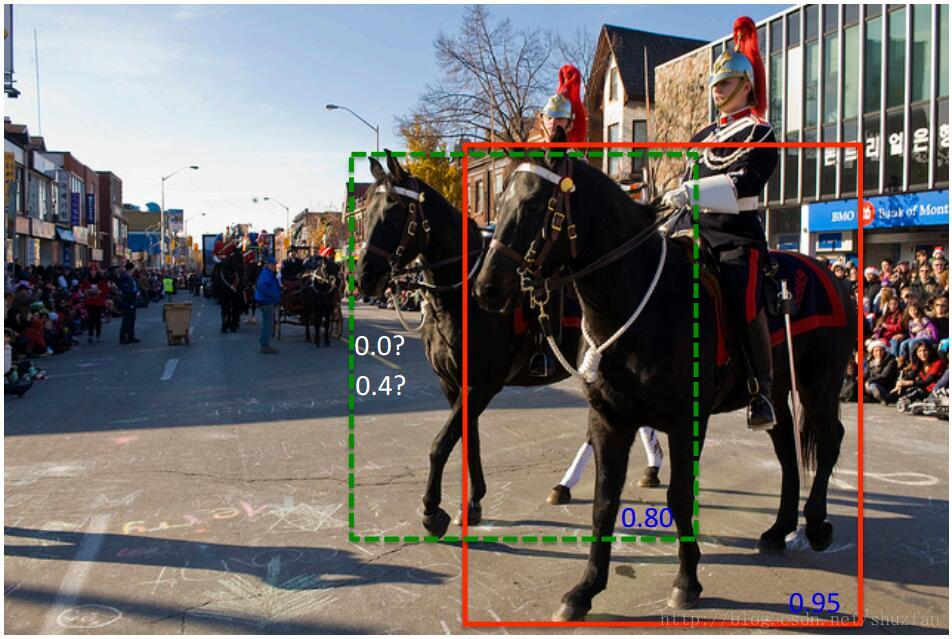
\includegraphics[width=\textwidth]{./Pictures/soft-nms.jpeg}	
	\caption{softnms}
\end{uscfigure}

传统的NMS处理方法可以通过以下的分数智重置函数(Rescoring Function)来表示:
\begin{equation}
	s_i = \left\{ 
		\begin{aligned}
		& s_i , &iou (M,b_i) < N_t \\
		& 0, 	&iou(M,b_i) \geq N_t
		\end{aligned}
		\right .
\end{equation}
在这个公式中,NMS采用了硬阈值来判断相邻检测框是否保留。但是,换一种方法,假设我们对一个与M高度重叠的检测框$b_i$的检测分数进行衰减,而非全部抑制。如果检测框$b_i$中包含不同于M中的物体,那么在检测阈值比较低的情况下,该物体并不会错过检测。但是,如果$b_i$中并不包含任何物体,即使在衰减过后,$b_i$的分数仍然较高,它还是会产生一个假阳性的结果,因此,在使用NMS做物体处理的时候,需要注意以下几点:

1、相邻检测框的检测分数应该被降低,从而减少假阳性结果,但是,衰减后的分数仍然应该比明显的假阳性结果要高。

2、通过较低的NMS重叠阈值来移除所有相邻检测框并不是最优解,并且很容易导致错过被检测物体,特别是在物体高度重叠的地方。

3、当NMS采用一个较高的重叠阈值时,平均准确率可能会相应降低。

值得注意的是,soft-NMS也是一种贪心算法,并不能保证找到全局最优的检测框分数重置。但是,soft-NMS算法是一种更加通用的非最大抑制算法,传统的NMS算法可以看做是它的一个采用不连续二值权重函数的特例。除了以上这两种分数重置函数,我们也可以考虑开发其他包含更多参数的分数重置函数,比如Gompertz函数等。但是它们在完成分数重置的过程中增加了额外的参数。
\subsubsection{数据增强}
采用数据扩增(Data Augmentation)可以提升SSD的性能,主要采用的技术有水平翻转(horizontal flip),随机裁剪加颜色扭曲(random crop \& color distortion),随机采集块域(Randomly sample a patch)获取小目标训练样本